\documentclass[11pt,a4paper]{article}
\usepackage{fontspec}
\defaultfontfeatures{Ligatures=TeX}
\setmainfont{Latin Modern Roman}
\setsansfont{Latin Modern Sans}
\setmonofont{Latin Modern Mono}
\IfFontExistsTF{Noto Serif CJK SC}
 {\newfontfamily\zhfont{Noto Serif CJK SC}}
 {\IfFontExistsTF{FandolSong-Regular}
   {\newfontfamily\zhfont{FandolSong-Regular}}
   {\PackageError{booster-paper}{Install Noto Serif CJK SC or FandolSong-Regular}{A CJK font is required only for the exact AI prompt.}}}
\usepackage[margin=1in,headheight=15pt,headsep=14pt]{geometry}
\usepackage{amsmath,amssymb,bm}
\usepackage{graphicx,booktabs,tabularx,longtable,array}
\usepackage{caption,subcaption}
\usepackage{enumitem,fancyhdr,microtype}
\usepackage[section]{placeins}
\usepackage{xurl}
\usepackage[hidelinks,unicode]{hyperref}
\usepackage[nameinlink,noabbrev]{cleveref}
% Replace only with the actual assigned team number.
\newcommand{\TeamNumber}{TBA}

% Automatically generated from frozen v15 evidence.
\newcommand{\Load}{140}
\newcommand{\EntryFuel}{98.308}
\newcommand{\LandingFuel}{38.942}
\newcommand{\ConsumedFuel}{137.250}
\newcommand{\RemainingFuel}{2.750}
\newcommand{\FlightTime}{364.203}
\newcommand{\Range}{347.624}
\newcommand{\Apogee}{144.782}
\newcommand{\ApogeeTime}{127.4}
\newcommand{\FirstIgnition}{260.00}
\newcommand{\EntryOff}{310.636}
\newcommand{\SecondIgnition}{315.636}
\newcommand{\PeakQ}{47.018}
\newcommand{\PeakN}{3.8002}
\newcommand{\PeakAlpha}{4.984}
\newcommand{\PeakTilt}{3.744}
\newcommand{\PeakGimbal}{2.745}
\newcommand{\PeakOmega}{3.418}
\newcommand{\PeakSlew}{4.613}
\newcommand{\FinalVr}{-1.0000}

\newcommand{\StageRows}{%
Unpowered ascent & 0.00--127.40 & 70.000--144.782 & 1666.7--1164.95 & 0.000 \\
Unpowered descent & 127.40--260.00 & 144.782--63.738 & 1165.0--1702.26 & 0.000 \\
Seven-engine entry burn & 260.00--310.64 & 63.738--15.478 & 1702.3--571.65 & 97.503 \\
Shutdown tail and coast & 310.64--315.64 & 15.478--13.136 & 571.7--577.81 & 0.805 \\
Three-engine landing burn & 315.64--364.20 & 13.136--0.032 & 577.8--1.00 & 38.942 \\
}

\newcommand{\FuelRows}{%
Initial carried propellant & 140.000 & 31.818 & 108.182 \\
Entry burn including shutdown tail & 98.308 & 22.343 & 75.965 \\
Landing burn to first foot contact & 38.942 & 8.850 & 30.091 \\
Remaining at first foot contact & 2.750 & 0.625 & 2.125 \\
}

\newcommand{\PerturbationRows}{%
$C_D-15\%$ & Sea-level foot event & 32.8 & -120.83 & 53.82 & Fail \\
$C_D-20\%$ & Sea-level foot event & 32.7 & -145.54 & 56.38 & Fail \\
$I_{sp}-2\%$ & Usable fuel exhausted & 462.6 & 1.59 & 44.79 & Fail \\
Wind $\times2$ & Planned end; no contact & 174.9 & -2.41 & 45.91 & Fail \\
Wind $\times3$ & Planned end; no contact & 321.9 & -3.78 & 44.77 & Fail \\
Combined & Sea-level foot event & 32.9 & -44.63 & 49.11 & Fail \\
}

\graphicspath{{../../results/figures/}{figures/}}
\captionsetup{font=normalsize,labelfont=normalfont,labelsep=period}
\captionsetup[table]{position=top}
\captionsetup[subfigure]{font=small,labelfont=normalfont,labelsep=space}
\setlist[itemize]{topsep=4pt,itemsep=2pt,parsep=0pt}
\setlist[enumerate]{topsep=4pt,itemsep=2pt,parsep=0pt}
\setlength{\parindent}{17pt}
\setlength{\parskip}{0pt}
\setlength{\emergencystretch}{1.5em}
\setcounter{tocdepth}{2}
\pagestyle{fancy}
\fancyhf{}
\fancyhead[L]{Problem A}
\fancyhead[R]{Team \TeamNumber}
\fancyfoot[C]{\thepage}
\renewcommand{\headrulewidth}{0.4pt}
\renewcommand{\footrulewidth}{0pt}
\newcommand{\dd}{\,\mathrm{d}}
\newcommand{\vect}[1]{\bm{#1}}
\newcommand{\er}{\vect e_r}
\newcommand{\et}{\vect e_t}
\newcommand{\eb}{\vect e_b}
\newcommand{\ep}{\vect e_p}
\newcommand{\kg}{\mathrm{kg}}
\newcommand{\ms}{\mathrm{m\,s^{-1}}}
\hypersetup{pdftitle={Conditional Propellant Requirements for Shipboard Recovery of a Seven-Engine Booster},pdfauthor={Team \TeamNumber},pdfsubject={Problem A: a conditional numerical study}}
\begin{document}
\hypersetup{pageanchor=false}
\pagenumbering{gobble}
\begin{center}
\vspace*{7mm}
{\LARGE\bfseries Conditional Propellant Requirements for\par Shipboard Recovery of a Seven-Engine Booster\par}
\vspace{5mm}
{\large Team \TeamNumber, Problem A\par}
\vspace{7mm}
{\large\bfseries Abstract\par}
\end{center}
\noindent
We study the recovery of a first-stage booster separating at 70 km altitude with a speed of 6,000 km/h, a dry mass of 130 t, a height of 65 m, and a diameter of 7 m. Because the problem does not specify propulsion, attitude control, or the initial velocity direction, we define a seven-engine reference scenario with an upward flight-path angle of $45^\circ$. A variable-mass model couples spherical-Earth translation, prescribed wind, aerodynamic drag, pitch motion, differential throttle, and finite engine response. CasADi/IPOPT generates candidate controls; an independently written Cartesian model verifies the resulting trajectory and first-foot-contact conditions.

The verified nominal candidate carries \Load\ t of liquid oxygen and methane. Its entry burn, including shutdown tail, consumes \EntryFuel\ t, and its landing burn consumes \LandingFuel\ t before first foot contact. The trajectory reaches an apogee of \Apogee\ km and makes first contact after \FlightTime\ s at a surface range of \Range\ km. Peak dynamic pressure is \PeakQ\ kPa, and the downward contact speed is approximately 1 m/s. Continuous replay detects and corrects a thrust-direction slew violation missed between optimization nodes.

These results establish a conditional nominal benchmark, not a global minimum or a robust recovery load. All six tested perturbations fail the unchanged open-loop plan. Assumed aerodynamic and mass properties, idealized pre-entry reorientation, and unmodeled three-dimensional, thermal, structural, and post-contact effects remain decisive limitations.
\clearpage
\hypersetup{pageanchor=true}
\pagenumbering{roman}
{\small\tableofcontents}
\clearpage
\pagenumbering{arabic}

\section{Introduction}
\label{sec:intro}
\subsection{Background and problem restatement}
A reusable booster must dissipate substantial mechanical energy while retaining enough control authority to reach a ship, become nearly upright, and make a manageable first contact. Bringing its center of gravity to a low speed is necessary, but the landing feet can still have significant velocities due to body rotation. A trajectory must therefore be interpreted together with engine dynamics, attitude motion, support geometry, and the conditions imposed on the deck.

The problem specifies a separation altitude of 70 km, a speed of 6,000 km/h, a dry mass of 130,000 kg, and vehicle dimensions of 65 m by 7.0 m. The propellants are liquid oxygen and methane, and the ship may be positioned conveniently \cite{problem}. The velocity direction, engine characteristics, aerodynamics, allowable loads, mass distribution, and landing-gear capabilities are not specified. A unique real-vehicle propellant requirement cannot be extracted from these data alone.

We adopt an explicitly upward initial flight-path angle $\gamma_0=45^\circ$ and seven virtual engines for this study. These are scenario choices, rather than additional facts inferred from the problem. The physical setting and assumed deployed geometry are illustrated in \cref{fig:mission}. The ship is selected once at the nominal downrange location. Its freedom of placement avoids a return-to-launch-site requirement; it does not remove the need to brake tangential motion.

\begin{figure}[htbp]
\centering
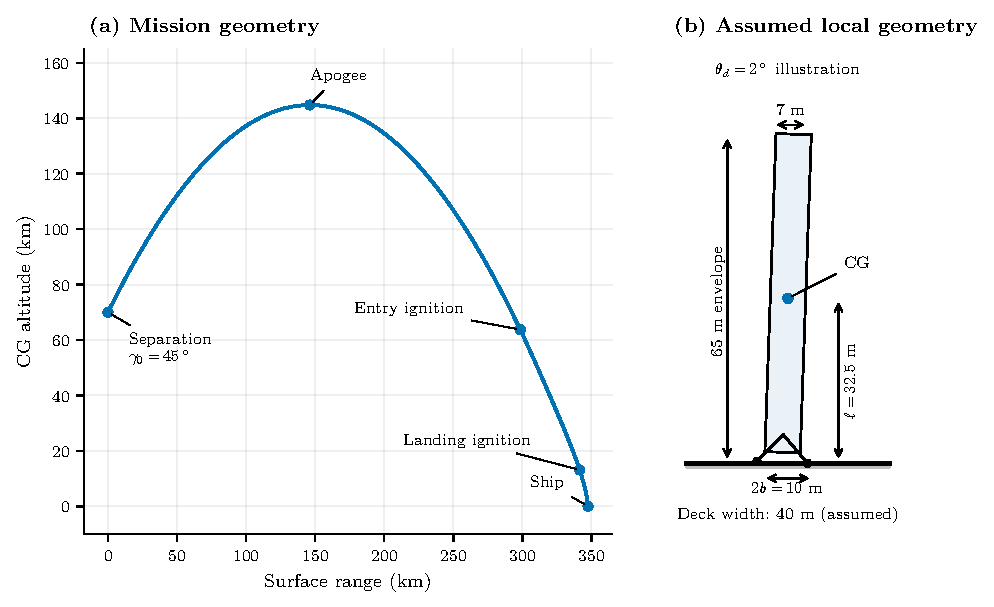
\includegraphics[width=\linewidth]{fig01_mission_geometry.pdf}
\caption{Recovery scenario and geometric definitions. (a) The mission trajectory and event locations are taken from the verified nominal replay. (b) The local geometry is an assumed construction at $2^\circ$ body tilt, not the nominal contact pose or a measured landing-leg design. The 2 m basal clearance and 10 m deployed foot span are study assumptions.}
\label{fig:mission}
\end{figure}

\subsection{Objectives and evidence boundaries}
The study has three objectives. First, formulate a transparent variable-mass reference model that retains gravity, Earth curvature, wind-relative drag, finite thrust response, and pitch motion. Second, find and independently verify a nominal recovery candidate within a stated engine and burn-sequence family. Third, identify which conclusions remain unsupported when the same controls face perturbations or when omitted recovery physics is considered.

We distinguish numerical verification from real-vehicle validation. Agreement between coordinate implementations or numerical integrators supports the computation of a specified model. It does not establish that an assumed drag coefficient, pressure center, engine map, or leg capacity represents the actual booster. Throughout the paper, a nominal pass refers only to the implemented checks under the reference assumptions.

\subsection{Methodology overview}
The workflow in \cref{fig:workflow} places trajectory optimization inside an independent acceptance process. We first classify the inputs and construct the environment and coupled equations. Direct multiple shooting with CasADi and IPOPT then produces local candidates. An independently written SI Cartesian implementation replays the actual engine response, detects foot events, and checks the constraints between control nodes. Rejected candidates return to the modeling or optimization stage; solver convergence alone is not acceptance.

\begin{figure}[htbp]
\centering
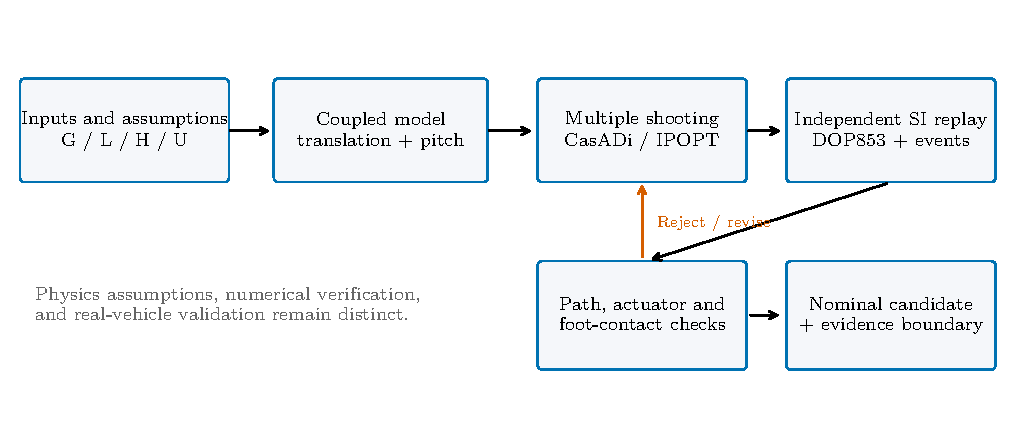
\includegraphics[width=\linewidth]{fig02_workflow.pdf}
\caption{Modeling, optimization, and independent acceptance workflow. G, L, H, and U distinguish problem data, literature support, adopted assumptions, and unresolved inputs. Independent replay is used to reject numerical candidates as well as to confirm them.}
\label{fig:workflow}
\end{figure}

\section{Assumptions and Notation}
\label{sec:assumptions}
\subsection{Reference scenario}
The evidence labels in \cref{tab:parameters} have the following meanings: G denotes information stated in the competition problem; L denotes literature constants or reference models; H denotes assumptions adopted for this study, including the specified $45^\circ$ scenario; U denotes inputs not established by the available information. An H value is not a certified engineering limit or an uncertainty bound.

\begin{table}[htbp]
\caption{Principal reference parameters and evidence status.}
\label{tab:parameters}
\small
\begin{tabularx}{\linewidth}{@{}p{.25\linewidth}p{.27\linewidth}cX@{}}
\toprule
Quantity & Reference value & Status & Basis or boundary\\
\midrule
Dry mass; dimensions & 130 t; 65 m; 7.0 m & G & Problem statement\\
Separation altitude; speed & 70 km; 1,666.667 m/s & G & Problem statement\\
Initial flight-path angle & $+45^\circ$ & H & Upward reference scenario\\
Engine number; reference thrust & 7; 1 MN per engine & H & Virtual engine family\\
Steady throttle; specific impulse & 0.3--1.1; 330 s & H & Constant across altitude\\
Oxygen/methane mass ratio & 3.4 & H & Total propellant includes both species\\
Earth radius; gravity parameter & $6.371\!\times\!10^6$ m; $3.986004418\!\times\!10^{14}$ m$^3$/s$^2$ & L/H & Literature constants; spherical non-rotating model\\
Density below about 86 km & USSA 1976 lower atmosphere & L & Geometric-to-geopotential conversion\\
Density above about 86 km & Exponential, 7 km scale height & H & Continuous extension to 220 km\\
Drag coefficient; area closure & $C_D=0.5$; attitude-dependent & H & Not a measured Mach/angle database\\
Wind & Prescribed along-track profile & H & No location-specific weather data\\
Inertia, pressure center, legs & Surrogates detailed below & H/U & Real properties remain unknown\\
\bottomrule
\end{tabularx}
\end{table}

The atmosphere is stationary except for a prescribed horizontal wind in the flight plane. Earth rotation, out-of-plane translation, yaw, roll, and ship motion are omitted. The initial carried mass includes dry mass and all remaining liquid oxygen and methane. No separate payload or returning upper stage is included.

Before the first entry ignition, reorientation is idealized: the body follows an incoming-flow reference without modeled actuator expenditure. At ignition, the pitch state is initialized consistently with that reference and zero inertial angular rate. The subsequent pitch and translation are integrated together. This assumption does not constitute a continuous reaction-control-system maneuver, and no RCS propellant requirement is established by it.

The supplied working document describes a 12-anchor $C_D(M)$ curve without providing the numerical anchors or executable scripts. We do not reconstruct an undocumented aerodynamic database from its claimed results. Instead, $C_D=0.5$ defines an auditable reference scenario. The new result must consequently not be interpreted as a like-for-like improvement over the document's earlier fuel estimates. Its force equations, contact definition, actuator constraints, and stage boundaries also differ from the present model.

\subsection{Notation and angle convention}
\begin{table}[htbp]
\caption{Main notation. All force equations are written in SI units.}
\label{tab:notation}
\small
\begin{tabularx}{\linewidth}{@{}lX@{}}
\toprule
Symbol & Definition\\
\midrule
$h,r,R,\phi,s$ & CG geometric altitude, geocentric radius, Earth radius, geocentric position angle, and surface range $s=R\phi$\\
$v_t,v_r,V,V_a$ & Local tangential and radial velocities, ground speed, and air-relative speed\\
$m,m_d,m_{p,0}$ & Total mass, dry mass, and initial total propellant\\
$T_i,T,D,q$ & Individual engine thrust, total parallel thrust, drag magnitude, and dynamic pressure\\
$\gamma,\theta,\beta,\delta$ & Flight-path angle; local body tilt; local thrust direction; thrust-to-body deflection\\
$\psi,\omega,I$ & Inertial body angle, inertial pitch rate, and transverse inertia\\
$\bar u,d,u_i$ & Mean throttle, differential throttle coordinate, and actual individual throttle\\
$\ell,a_i,b$ & Axial engine lever, lateral engine coordinate, and deployed foot half-span\\
$n_\Sigma$ & Sum-of-force-magnitudes budget normalized by $mg_0$\\
\bottomrule
\end{tabularx}
\end{table}

The local thrust direction $\beta$ is measured from the upward radial direction toward increasing downrange. Thus $\beta<0$ gives an upstream component. The body axis points from the engine end toward the nose, and $\delta=\beta-\theta$. Inertial angle is $\psi=\theta+\phi$. Ground flight-path angle is $\gamma=\operatorname{atan2}(v_r,v_t)$ and is distinct from body tilt.

\section{Physical Analysis of the Recovery Process}
\label{sec:physical}
\subsection{Initial ascent, gravity, and Earth curvature}
The specified separation speed is $V_0=6000/3.6$ m/s. An upward $45^\circ$ flight-path angle gives
\begin{equation}
 v_{t,0}=V_0\cos45^\circ=1178.5113\ \ms,\qquad
 v_{r,0}=V_0\sin45^\circ=1178.5113\ \ms.
\label{eq:initial}
\end{equation}
The booster therefore rises before it begins descending. Its speed initially decreases, but it retains substantial tangential motion at apogee.

At separation, $h_0/R\simeq0.011$ and the curvature contribution $v_{t,0}^2/(R+h_0)$ is about $0.216$ m/s$^2$. This is not negligible over a several-hundred-kilometer flight. The initial kinetic energy per unit mass is about 1.39 MJ/kg, and the potential decrease from 70 km to sea level is about 0.68 MJ/kg. Curvature and altitude-dependent gravity are therefore retained rather than absorbed into a planar constant-gravity approximation.

A vacuum central-force check gives an apogee near 144.786 km at 127.401 s. The nominal atmospheric calculation gives \Apogee\ km at approximately \ApogeeTime\ s. The close agreement is consistent with the low density on the initial high-altitude arc; it does not imply that drag is unimportant later in descent.

Central gravity conserves specific angular momentum in vacuum,
\begin{equation}
 (R+h)v_t=(R+h_0)v_{t,0},
\label{eq:angularmomentum}
\end{equation}
and does not dissipate tangential motion. A convenient ship position removes an imposed return maneuver, while drag and upstream thrust still supply the required angular-momentum change.

\subsection{Atmospheric density and prescribed wind}
Earth constants are drawn from NASA and IERS reference values \cite{earth,iers}. Below about 86 km geometric altitude, density is computed from the lower-atmosphere formulation of USSA 1976 \cite{ussa}. Geometric altitude $h$ is converted to geopotential height $H$ using
\begin{equation}
 H=\frac{R_a h}{R_a+h},\qquad R_a=6{,}356{,}766\ \mathrm{m}.
\end{equation}
Within each layer, atmospheric temperature is $T_a=T_b+L_b(H-H_b)$ and
\begin{equation}
 p=\begin{cases}
 p_b\left(T_b/T_a\right)^{g_0/(R_{\rm air}L_b)},&L_b\ne0,\\
 p_b\exp[-g_0(H-H_b)/(R_{\rm air}T_b)],&L_b=0,
 \end{cases}
 \qquad \rho=\frac{p}{R_{\rm air}T_a},
\label{eq:ussa}
\end{equation}
where $R_{\rm air}=8314.32/28.9644$ J/(kg K). The atmospheric conversion radius $R_a$ is not substituted for the gravitational radius $R$.

To cover the upward arc, the density is extended continuously above the lower-model boundary $h_b\simeq86$ km:
\begin{equation}
 \rho(h)=\rho(h_b)\exp\left[-\frac{h-h_b}{7000\ \mathrm{m}}\right],\qquad h>h_b.
\label{eq:extension}
\end{equation}
This extension is an H-class approximation, not the full high-altitude composition model of USSA 1976. Maximum nominal dynamic pressure above 86 km is about 8.54 Pa, whereas the primary screening limit is 50,000 Pa. Most aerodynamic braking and load screening therefore occur well below the extrapolated region.

Wind follows the supplied height anchors: 8 m/s below 0.1 km, 15 m/s at 2 km, 35 m/s at 11 km, and 20 m/s at 20 km, with linear interpolation. Above 20 km,
\begin{equation}
 w(h)=20\exp[-(h_{\rm km}-20)/15]\ \ms.
\label{eq:wind}
\end{equation}
The profile is an illustrative along-track scenario, not measured weather, an ERA5 realization, or an independently justified climatological mean. Density and wind are shown in \cref{fig:environment}.

\begin{figure}[htbp]
\centering
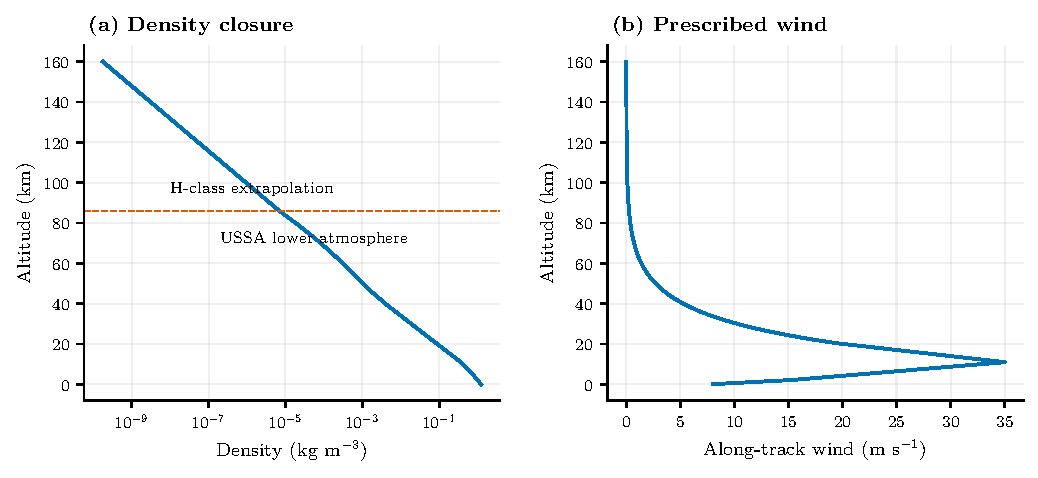
\includegraphics[width=\linewidth]{fig03_environment.pdf}
\caption{Environmental closure. (a) The lower-atmosphere density is joined continuously to an explicitly assumed exponential extension above about 86 km. (b) The prescribed along-track wind follows the supplied anchors. Neither curve represents date- and location-specific atmospheric observations.}
\label{fig:environment}
\end{figure}

\subsection{Air-relative drag and dynamic pressure}
With local unit vectors $\et$ and $\er$, air-relative velocity is
\begin{equation}
 \vect v_a=\vect v-w(h)\et,\qquad V_a=|\vect v_a|,
 \qquad q=\tfrac12\rho V_a^2.
\end{equation}
Let $\eb$ point toward the vehicle nose and $\ep$ be its clockwise-normal unit vector. Define inflow angle by
\begin{equation}
 \cos\alpha=-\frac{\vect v_a\cdot\eb}{V_a},\qquad
 \sin\alpha=\frac{\vect v_a\cdot\ep}{V_a}.
\end{equation}
The engine-end-first orientation has $\alpha\simeq0$ under this convention. The effective-area closure is
\begin{equation}
 A_{\rm eff}=A\cos^2\alpha+(65\times7)\sin^2\alpha,
 \qquad A=\frac{\pi(7\ \mathrm{m})^2}{4}=38.48451\ \mathrm{m}^2,
\label{eq:area}
\end{equation}
followed by
\begin{equation}
 D=qC_DA_{\rm eff},\qquad \vect F_a=-D\frac{\vect v_a}{V_a},\qquad C_D=0.5.
\label{eq:drag}
\end{equation}
This projection-inspired area law is a modeling assumption. It does not supply a measured drag/lift/moment database. Drag coefficients depend on geometry and flow conditions \cite{drag}, and retropropulsion can substantially alter the local flow \cite{retro}. No experimental coefficients from a different vehicle are transferred into this model.

The pressure threshold implies $V_a\le\sqrt{2q_{\rm lim}/\rho}$, with no $C_D$ factor. Moreover,
\begin{equation}
 \dot q=\tfrac12\dot\rho V_a^2+\rho\vect v_a\cdot\dot{\vect v}_a.
\end{equation}
Increasing density and finite engine response mean that a full-throttle trigger near the pressure limit cannot, by itself, guarantee future constraint satisfaction. We instead constrain and independently replay the trajectory.

\section{Coupled Variable-Mass and Pitch Model}
\label{sec:model}
\subsection{Translation and mass flow}
Let $r=R+h$ and $s=R\phi$. For parallel active engine vectors,
\begin{align}
 \dot h&=v_r,&\dot\phi&=\frac{v_t}{r},&\dot s&=\frac{Rv_t}{r},\\
 \dot v_t&=\frac{T\sin\beta+F_{a,t}+F_{j,t}}{m}-\frac{v_rv_t}{r},
 \label{eq:vt}\\
 \dot v_r&=\frac{T\cos\beta+F_{a,r}+F_{j,r}}{m}-\frac{\mu}{r^2}+\frac{v_t^2}{r},
 \label{eq:vr}\\
 \dot m&=-\frac{\sum_i T_i}{v_e},&
 v_e&=I_{sp}g_0,&T_i&=10^6u_i\ \mathrm{N},
\label{eq:mass}
\end{align}
with $I_{sp}=330$ s and $g_0=9.80665$ m/s$^2$. The curvature terms in \cref{eq:vt,eq:vr} arise from the rotating local basis. The small selected mass-flow transport force $\vect F_j$ is defined below.

Specific impulse relates effective thrust to total expelled propellant \cite{isp}. In general, nozzle pressure and momentum contribute to thrust. Here $v_e=3236.1945$ m/s is an effective exhaust velocity; without nozzle exit area and pressure, it cannot be identified with a separately verified gas exit speed. Constant $I_{sp}$ and reference thrust across altitude are virtual-engine assumptions.

With oxygen/methane ratio 3.4,
\begin{equation}
 m_{\rm CH_4}=\frac{m_p}{4.4},\qquad
 m_{\rm LOX}=\frac{3.4m_p}{4.4}.
\end{equation}
Unusable propellant remains in the total mass. Its assigned amount is $0.005m_{p,0}$, and usable mass is
\begin{equation}
 m_{\rm use}=m-m_d-0.005m_{p,0}.
\label{eq:usable}
\end{equation}
The terminal reserve target is one second of maximum three-engine thrust,
\begin{equation}
 m_{\rm res}=\frac{3.3\times10^6\ \mathrm{N}\times1\ \mathrm{s}}{v_e}
 \simeq1019.72\ \kg,
\label{eq:reserve}
\end{equation}
with a further 50 kg optimization buffer. This is an assigned mass margin, not demonstrated disturbance tolerance.

\subsection{Engine allocation and pitch dynamics}
The first burn uses all seven engines. The second uses the center engine and a diametrically opposed pair of ring engines. At low speed, one engine at its assumed 1.1 MN maximum cannot hover against the 130 t dry weight, approximately 1.28 MN. Three engines span 0.9--3.3 MN, whereas all seven at minimum steady throttle provide 2.1 MN. Selecting three engines provides a more suitable terminal throttle range. It is not a proof that no brief single-engine ballistic contact or alternative engine sequence could be feasible.

For pitch-plane lateral coordinates,
\begin{equation}
 a_i=(0,2.5,1.25,-1.25,-2.5,-1.25,1.25)\ \mathrm{m}
\end{equation}
for entry, and $(0,2.5,-2.5)$ m for landing, we allocate actual throttle as
\begin{equation}
 u_i=\bar u+\frac{a_i}{2.5\ \mathrm{m}}d,
 \quad T=\sum_iT_i,\quad S_1=\sum_i a_iT_i,\quad S_2=\sum_i a_i^2T_i.
\label{eq:allocation}
\end{equation}
The out-of-plane symmetry is assumed; yaw and roll are not solved.

The inertial angle and local tilt obey
\begin{equation}
 \dot\psi=\omega,\qquad \dot\theta=\omega-\frac{v_t}{r},
 \qquad \beta=\theta+\delta.
\end{equation}
Use the effective cylinder inertia $I=mK^2$, where
\begin{equation}
 K^2=\frac{65^2+3(3.5)^2}{12}=355.145833\ \mathrm{m}^2.
\end{equation}
For clockwise-positive angles and engine mounts $-\ell\eb+a_i\ep$, with $\ell=32.5$ m,
\begin{align}
 I\dot\omega&=M_T+M_a+M_j+M_{gg},\\
 M_T&=-\ell T\sin\delta-S_1\cos\delta,\\
 M_a&=-5\ \mathrm{m}\,D\sin\alpha
       -\frac{qA(65\ \mathrm{m})^2}{2V_a}\omega,\\
 M_j&=-\frac{T(\ell^2-K^2)+S_2}{v_e}\omega,\\
 M_{gg}&=-\frac{3\mu}{2r^3}\left[I-\tfrac12m(3.5\ \mathrm{m})^2\right]\sin2\theta.
\label{eq:pitch}
\end{align}
The pressure center is assumed 5 m above the CG and the nondimensional damping coefficient is one. These choices, together with the equivalent inertia, are H-class surrogates.

Within the selected fixed-geometry, point-outlet approximation, the translational correction is
\begin{equation}
 \vect F_j=\frac{\omega}{v_e}\left(\ell T\ep+S_1\eb\right).
\label{eq:jetforce}
\end{equation}
The term $M_j$ combines the selected angular-momentum outflow and the assigned inertia evolution; the same inertia-rate term must not be added again. Variable-mass dynamics depend on internal flow and mass distribution \cite{variablemass}. Equations \eqref{eq:pitch}--\eqref{eq:jetforce} do not model slosh, true CG migration, a finite nozzle radius, or internal liquid momentum, and are not presented as a complete liquid-rocket multibody model.

\subsection{Finite engine response}
An ignition command does not provide instantaneous full thrust. With elapsed time $\tau$ after the command, the startup model is
\begin{equation}
 u_{\rm on}(\tau)=
 \begin{cases}
 0,&\tau\le0.5\ \mathrm{s},\\
 (\tau-0.5\ \mathrm{s})/(1\ \mathrm{s}),&0.5<\tau\le1.5\ \mathrm{s},\\
 1.1-0.1\exp[-(\tau-1.5\ \mathrm{s})/(0.1\ \mathrm{s})],&\tau>1.5\ \mathrm{s}.
 \end{cases}
\label{eq:startup}
\end{equation}
The stable controlled segment starts 1.6 s after ignition. Piecewise-linear actual throttle is constrained together with its effective command,
\begin{equation}
 u_{i,c}=u_i+(0.1\ \mathrm{s})\dot u_i,\qquad
 0.3\le u_i,u_{i,c}\le1.1,\quad |\dot u_i|\le1\ \mathrm{s}^{-1}.
\label{eq:actuator}
\end{equation}
The lower throttle bound applies to steady enabled engines. Startup and shutdown may pass below 0.3.

For shutdown from $u_0$, set $s_0=\max(u_0-0.1,0)\times1$ s. The actual response is
\begin{equation}
 u_{\rm off}(\tau)=\begin{cases}
 u_0-\tau/(1\ \mathrm{s}),&0\le\tau\le s_0,\\
 \min(u_0,0.1)\exp[-(\tau-s_0)/(0.1\ \mathrm{s})],&\tau>s_0.
 \end{cases}
\end{equation}
Shutdown tail is integrated into the mass and force histories rather than discarded at the command. Any additional real ignition or cutoff behavior would require engine data not available here.

\subsection{First-foot-contact geometry}
In a local static deck frame, let $H_c$ be CG height and $\theta_d$ body tilt relative to deck normal. For $b=5$ m and $\ell=32.5$ m,
\begin{align}
 \vect r_{f,\pm}&=\vect r_{CG}-\ell\eb\pm b\ep,\\
 h_{f,\min}&=H_c-\ell\cos\theta_d-b|\sin\theta_d|,
\label{eq:footheight}\\
 \vect v_{f,\pm}&=\vect v_{CG}+\omega(-\ell\ep\mp b\eb).
\label{eq:footvelocity}
\end{align}
A CG-height event alone cannot replace \cref{eq:footheight,eq:footvelocity}. At $2^\circ$ tilt, for example, the feet differ in height by $2b\sin2^\circ\simeq0.349$ m, so their loading is generally nonsimultaneous.

The assumed non-supporting body envelope spans axial coordinates 2--65 m above the foot-plane center, with radius 3.5 m. Side outlines are sampled at 1 m spacing including the ends. For the present planar line segments, height relative to a static deck plane is affine along each edge, so endpoint minima also cover edge interiors. The resulting geometry is only a proxy for actual nozzles, legs, protrusions, and deployment states.

\section{Constrained Trajectory Optimization}
\label{sec:optimization}
\subsection{Burn sequence and objective}
The strategy family consists of an initial unpowered arc, a seven-engine entry burn, a shutdown command, a restart command at least five seconds later, and a three-engine landing burn. The interval separates commands; it is not a full zero-thrust interval because the first engines decay continuously and the restarted engines have finite buildup.

CasADi provides automatic differentiation, and IPOPT solves the nonlinear multiple-shooting problem \cite{casadi,ipopt}. Free-load searches minimize initial propellant in tonnes plus a small control regularization,
\begin{equation}
 J=\frac{m_0-m_d}{1000\ \kg}
    +10^{-5}\sum_k(d_k^2+\delta_k^2),
\end{equation}
where angles in the regularizer are in radians. For a fixed load, the fuel term becomes $0.01(m_0-m_f)/(1000\ \kg)$ with the same regularizer. These objectives define a local numerical search, not a proof of a global fuel minimum.

The final accepted branch fixes first ignition at 260 s and initial propellant at 140 t. Phase durations and control nodes are optimized. Entry and landing steady segments are bounded to 5--110 s and 5--160 s; the command gap is 5--100 s, and final time is 260--500 s. Preliminary searches also allowed first ignition between 230 and 300 s, but returned distinct local branches. Those runs do not establish a converged global ranking.

\subsection{Path and terminal requirements}
\begin{table}[htbp]
\caption{Selected study constraints. Numerical limits are H-class screening targets.}
\label{tab:constraints}
\small
\begin{tabularx}{\linewidth}{@{}p{.34\linewidth}XX@{}}
\toprule
Quantity & Optimization setting & Independent acceptance\\
\midrule
Dynamic pressure & $q\le47$ kPa & $q\le50$ kPa\\
Non-gravity force budget & $n_\Sigma\le3.8$ without the small $|F_j|$ addition & $n_\Sigma\le4$ including $|F_j|$\\
High-pressure inflow & Conservative continuous screen & $|\alpha|\le5^\circ$ where $q\ge10$ kPa\\
Low-altitude body tilt & $3.5^\circ$ low-altitude bound with transition & $|\theta|\le5^\circ$ at $h\le232.5$ m\\
Individual steady throttle & Actual and implied command in 0.3--1.1 & Same; startup/shutdown excepted\\
Gimbal amplitude and slew & $6^\circ$; $20^\circ$/s & Checked from controls\\
Inertial thrust-direction slew & $4.5^\circ$/s at modeled substeps & $5^\circ$/s in controlled burn segments\\
Inertial body rate & $10^\circ$/s & Modeled pitch history\\
First-contact state & $v_t=0$, $v_r=-1$ m/s, $\theta=\omega=0$ & Foot vertical speed $\le2$ m/s, horizontal speed $\le0.5$ m/s\\
Contact pose & Upright target & Tilt $\le2^\circ$; rate $\le0.5^\circ$/s\\
Mass and reserve & Unusable fraction, reserve, 50 kg buffer & Reserve and usable mass checked\\
Deck and envelope & Nominal endpoint target & Feet within $\pm18$ m; body does not touch first\\
\bottomrule
\end{tabularx}
\end{table}

The conservative replay force budget is
\begin{equation}
 n_\Sigma=\frac{T+D+|\vect F_j|}{mg_0}.
\label{eq:nsum}
\end{equation}
It is a sum-of-magnitudes bound on non-gravitational acceleration, not a measured structural load factor or a flight-path normal acceleration. Dynamic pressure and this budget are coupled by $D=qC_DA_{\rm eff}$.

For inflow, optimization uses
\begin{equation}
 \max(q-1000\ \mathrm{Pa},0)(1-\cos\alpha)
 \le9000\ \mathrm{Pa}(1-\cos5^\circ).
\label{eq:inflowscreen}
\end{equation}
This is at least as restrictive as $5^\circ$ once $q\ge10$ kPa, and becomes inactive below 1 kPa. The release at low pressure permits an upright vehicle to encounter horizontal sea wind near contact without imposing an inappropriate incoming-flow alignment.

The terminal vertical thrust is limited to 0.95 times local weight. This helps define a downward-approach reference, but does not demonstrate stable support after contact. The reserve requirement is an accounting condition, not a replacement for perturbation tests.

\subsection{Discretization and independent acceptance}
The final model has 160 unpowered-arc intervals and 60 control intervals in each steady powered phase. Each powered interval uses four RK4 substeps. Startup is resolved at 0.05 s nodes, while the first two seconds after shutdown use 0.0125 s substeps. IPOPT uses tolerance $10^{-7}$, acceptable tolerance $10^{-5}$, and a final fixed-load iteration budget of 1000.

The optimizer scales distance, velocity, mass, and thrust to km, km/s, tonnes, and MN. Independent replay instead uses SI Cartesian position and velocity, inertial body angle, and pitch rate. It applies DOP853 with explicit control breakpoints, continuous foot-clearance and usable-mass events, 0.05 s output sampling, and a maximum step of 0.1 s \cite{scipy,ivp}. Step halving to 0.05 s supplies a further comparison.

Independent replay detected a slew violation in an earlier candidate. Inertial thrust direction briefly changed at about $5.13^\circ$/s between checks, although the optimizer used a $5^\circ$/s limit. That candidate was rejected. Tightening the optimization limit to $4.5^\circ$/s and re-solving produced the final controls. Thus the independent calculation changed which numerical candidate could be accepted.

\section{Nominal Recovery Results}
\label{sec:results}
\subsection{Trajectory and event sequence}
The verified candidate carries \Load\ t of propellant, for a separation total mass of 270 t. \Cref{fig:trajectory} shows its trajectory, ground speed, flight-path angle, and CG altitude. Orange shading marks the seven-engine command interval and green shading the final burn. The initial upward arc is a direct consequence of \cref{eq:initial}, rather than a control action.

\begin{figure}[htbp]
\centering
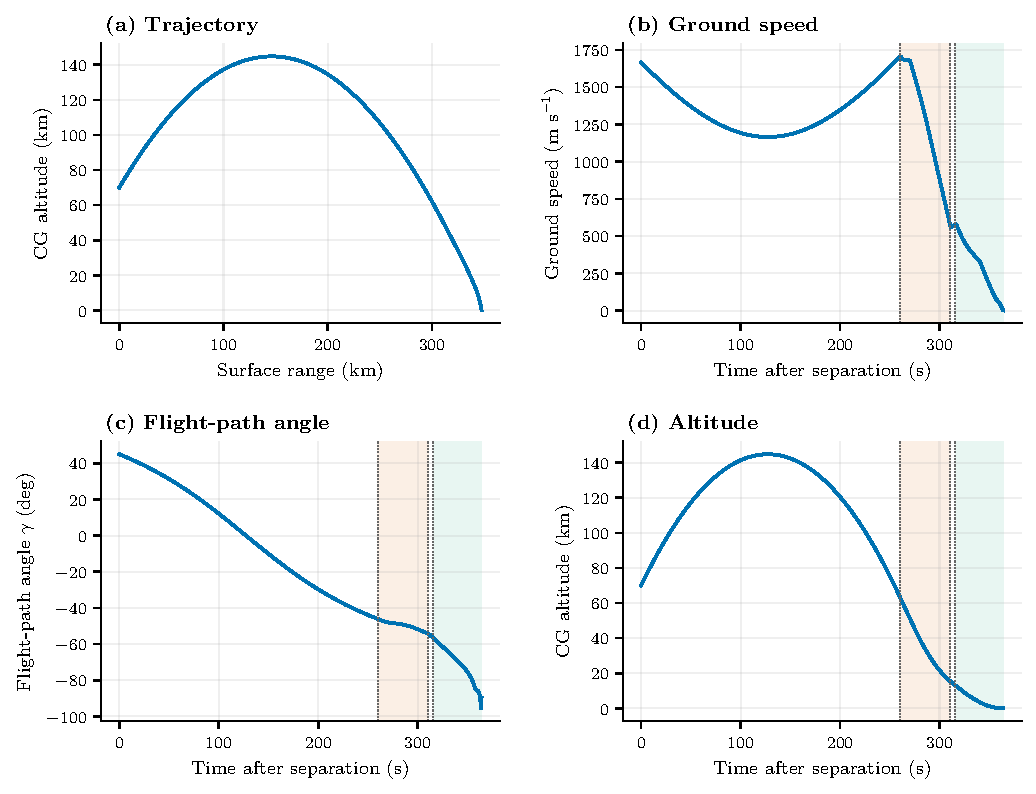
\includegraphics[width=\linewidth]{fig04_trajectory.pdf}
\caption{Nominal trajectory from independent SI replay: (a) surface range and CG altitude, (b) ground speed, (c) local flight-path angle, and (d) CG altitude versus time. The booster first ascends to \Apogee\ km and then descends. Colored intervals indicate the entry and landing burns. First foot contact occurs with CG height near 32.5 m, not zero CG altitude.}
\label{fig:trajectory}
\end{figure}

\begin{table}[htbp]
\caption{Nominal phases and independently replayed states. The tail/coast consumption is assigned to the first burn in total fuel bookkeeping.}
\label{tab:stages}
\small
\setlength{\tabcolsep}{3.5pt}
\begin{tabular}{@{}lrrrr@{}}
\toprule
Phase & \shortstack{Time\\(s)} & \shortstack{Altitude\\(km)} & \shortstack{Ground speed\\(m/s)} & \shortstack{Propellant\\(t)}\\
\midrule
\StageRows
\bottomrule
\end{tabular}
\end{table}

The first ignition occurs at 260 s and approximately 63.74 km altitude, after the booster has passed apogee. The seven-engine burn continues to about 15.5 km before the off command at \EntryOff\ s. The three-engine restart command is issued at \SecondIgnition\ s and about 13.1 km altitude. First foot contact follows at \FlightTime\ s, at a surface range of \Range\ km.

The first burn therefore performs substantially more braking than a short, prescribed 75--55 km entry pulse. Comparing its fuel directly with the supplied document's 40--44 t entry-pulse number would compare different stage definitions. Likewise, a nearly linear segment of an altitude plot does not establish constant descent speed; the velocity and force histories must be examined explicitly.

\subsection{Thrust allocation and attitude history}
\Cref{fig:controls} shows actual engine throttles, body and thrust directions, angular rates, and total thrust. Entry thrust has an upstream component and an upward component. During the final burn, tangential speed is removed while the body becomes nearly upright. Body attitude and thrust direction differ through the gimbal angle; they are not negatives of one another.

\begin{figure}[htbp]
\centering
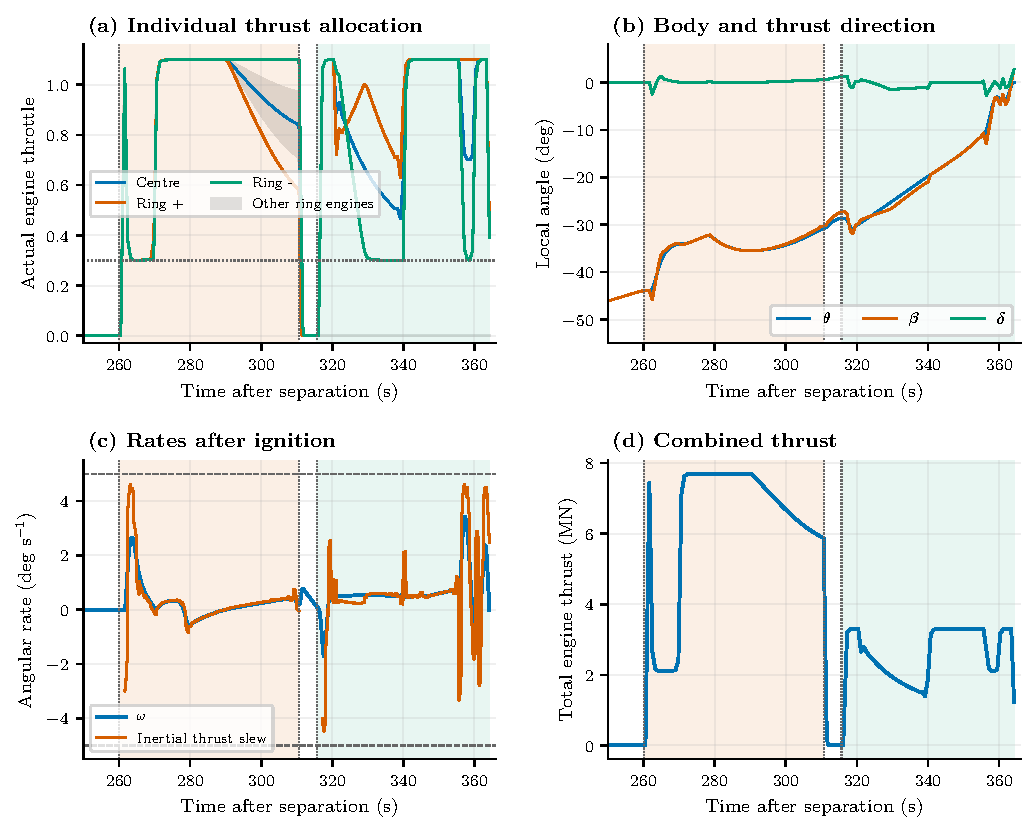
\includegraphics[width=\linewidth]{fig05_controls.pdf}
\caption{Control and pitch histories after the first ignition. (a) Actual engine throttles include finite buildup and shutdown decay; values below 0.3 during those transients are permitted. (b) Body tilt $\theta$, thrust direction $\beta$, and relative deflection $\delta$ are distinct. (c) The thrust slew trace is shown for the controlled steady segments, with the $5^\circ$/s acceptance limits. (d) Combined engine thrust includes the shutdown tail.}
\label{fig:controls}
\end{figure}

Peak combined thrust is approximately 7.699 MN in the seven-engine phase and 3.300 MN in the three-engine phase. These are peaks, not constant values to be multiplied by a burn duration. Maximum gimbal amplitude is \PeakGimbal$^\circ$, maximum inertial body rate is \PeakOmega$^\circ$/s, and the independently sampled peak inertial thrust slew in controlled segments is \PeakSlew$^\circ$/s. The time histories are supported by the individual steady-command and throttle-rate checks.

The nominal result does not establish a real reorientation design. The long pre-entry interval still uses the assumed ideal reference, and the post-ignition moments depend on surrogate mass and aerodynamic properties. Feasible motion of this mathematical model is not evidence that an unspecified hardware actuator can realize the same motion.

\subsection{Propellant allocation and mass closure}
\begin{table}[htbp]
\caption{Nominal propellant bookkeeping for oxygen/methane ratio 3.4. Values are rounded; unrounded data are retained in the calculation record.}
\label{tab:fuel}
\small
\begin{tabularx}{\linewidth}{@{}Xrrr@{}}
\toprule
Quantity & Total (t) & Methane (t) & Oxygen (t)\\
\midrule
\FuelRows
\bottomrule
\end{tabularx}
\end{table}

The total consumption to first foot contact is \ConsumedFuel\ t, leaving \RemainingFuel\ t. The latter includes 0.700 t assigned unusable propellant; approximately 2.050 t remains usable. This exceeds the 1.020 t nominal reserve target, but the difference is not a demonstrated emergency-maneuver allowance.

\begin{figure}[htbp]
\centering
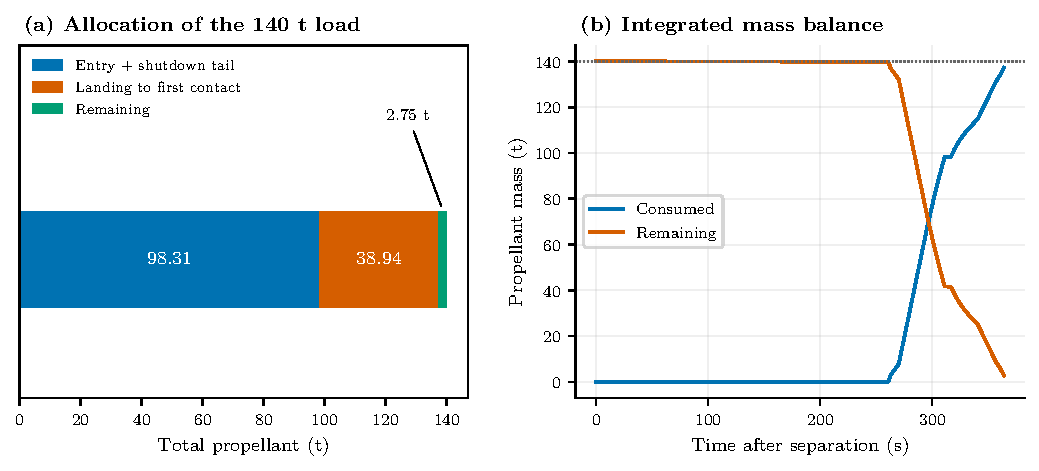
\includegraphics[width=\linewidth]{fig07_propellant.pdf}
\caption{Mass closure for the single verified \Load\ t reference case. (a) First-burn consumption includes the shutdown tail up to the second ignition. (b) Integrated consumed and remaining total propellant. Carried mass, consumed mass, methane mass, and usable reserve are separate quantities. No family of unverified low-load trajectories is implied by this figure.}
\label{fig:fuel}
\end{figure}

An exact scalar closure under constant $v_e$ is
\begin{equation}
 \Delta v_T\equiv\int_0^{t_f}\frac{T}{m}\dd t
 =v_e\ln\frac{m_0}{m_f}.
\label{eq:rocket}
\end{equation}
It is the integrated thrust-acceleration magnitude, not the net speed change or an independently selected passive impact speed. Gravity, drag, steering, and changing mass all affect the trajectory over which this thrust is expended. Equation \eqref{eq:rocket} therefore checks mass-flow accounting rather than replacing trajectory integration.

\subsection{Selected nominal checks}
\begin{figure}[htbp]
\centering
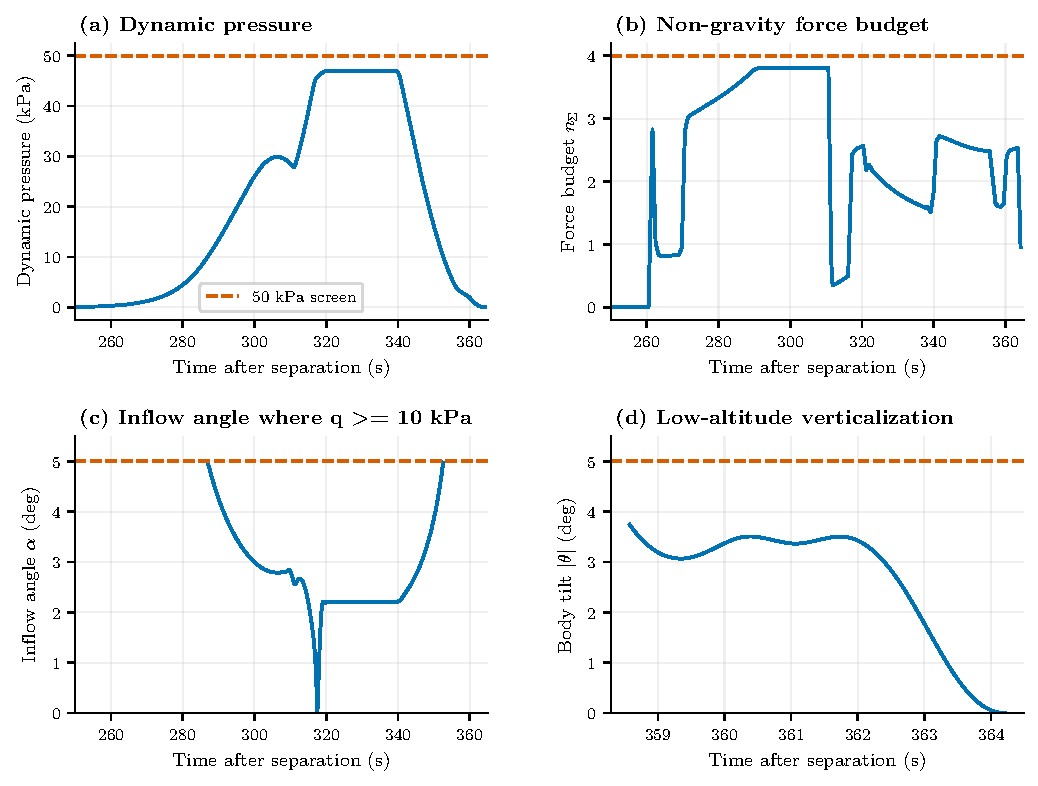
\includegraphics[width=\linewidth]{fig06_screens.pdf}
\caption{Selected H-class screening requirements. (a) Peak dynamic pressure remains below 50 kPa. (b) The non-gravity sum-of-magnitudes budget remains below four. (c) Inflow angle is shown only where $q\ge10$ kPa. (d) Low-altitude tilt is evaluated at CG height $h\le232.5$ m. Passing these checks does not establish structural, thermal, or post-contact safety.}
\label{fig:screens}
\end{figure}

Peak dynamic pressure is \PeakQ\ kPa and peak $n_\Sigma$ is \PeakN. The high-pressure inflow angle reaches \PeakAlpha$^\circ$, while the largest low-altitude body tilt is \PeakTilt$^\circ$. At nominal contact, the body is nearly upright, the foot horizontal speeds are approximately $1.5\times10^{-4}$ m/s in magnitude, and both foot vertical speeds are near $-1$ m/s. The main-cylinder proxy remains about 2 m above the assumed static deck at first foot contact.

The ship is placed at the nominal CG surface projection once. The feet lie approximately 5 m on either side of the chosen center, within the assigned 18 m safe half-width. A free nominal ship position does not establish navigation accuracy or recovery on a moving deck. The spherical sea-level foot event differs from the local tangent-plane event by only about two micrometers in height for this nominal geometry; that small geometrical difference is unrelated to real waves or ship motion.

\section{Numerical Verification and Perturbation Response}
\label{sec:verification}
\subsection{Implementation and integration checks}
Verification addresses three separate issues: implementation consistency, integration resolution, and feasibility of the recorded controls in the specified model. It does not convert scenario assumptions into measured inputs.

The density implementations agree over 109 sampled heights through 220 km, including the upper extension, to a maximum relative difference of about $1.67\times10^{-10}$. A vacuum central-force check conserves specific energy and angular momentum to the numerical precision reported in \cref{tab:verification}. Eighty random states compare the SI Cartesian derivatives, transformed back to local quantities, with the independently coded scaled equations. The largest component difference is approximately $2.46\times10^{-10}$ in the corresponding SI units.

\begin{table}[htbp]
\caption{Numerical verification evidence for the specified model. Small numerical discrepancies are not physical uncertainty bounds.}
\label{tab:verification}
\small
\begin{tabularx}{\linewidth}{@{}p{.36\linewidth}X@{}}
\toprule
Check & Observed result\\
\midrule
Density implementations, 109 heights & Maximum relative difference $1.67\times10^{-10}$\\
Vacuum energy invariant & Maximum specific-energy drift $3.73\times10^{-8}$ J/kg\\
Vacuum angular momentum & Maximum drift $1.05\times10^{-5}$ m$^2$/s\\
Independent coordinate RHS, 80 states & Maximum component difference $2.46\times10^{-10}$ in corresponding SI units\\
Step halving, 0.1 to 0.05 s & $\Delta t_f=4.50\times10^{-6}$ s; $\Delta s_f=2.97\times10^{-5}$ m; $\Delta v_{r,f}=2.37\times10^{-6}$ m/s; $\Delta m_f=1.72\times10^{-3}$ kg\\
Individual engine commands & Actual throttle, implied command, slew and gimbal checks pass\\
Startup/shutdown response & Response continuity and shutdown-flow integrals pass\\
Inter-node thrust slew & Earlier $5.13^\circ$/s candidate rejected; revised peak \PeakSlew$^\circ$/s\\
\bottomrule
\end{tabularx}
\end{table}

The independent maximum-step comparison gives much smaller discrepancies than the uncertainties in drag, inertia, or engine maps. However, a fine integration of a fixed control history is not a control-grid convergence proof. Different coarse/refined and free-ignition searches returned distinct local branches. Resource-terminated runs were not counted as successful optimizations. The final claim is reproducibility and nominal acceptance of the recorded branch, rather than a verified global optimum.

\subsection{Load search and its interpretation}
\begin{table}[htbp]
\caption{Discrete load-search evidence. Failure within a finite local search budget is not a proof of physical infeasibility.}
\label{tab:loadsearch}
\small
\begin{tabularx}{\linewidth}{@{}rXX@{}}
\toprule
Load (t) & Numerical search & Interpretation\\
\midrule
90, 100, 110, 120, 130 & 30 intervals per powered phase; 90 IPOPT iterations for each tested warm start & No strictly accepted solution returned within the assigned budget\\
140 & 60 intervals per powered phase; final fixed-260 s branch with slew margin and independent replay & Selected nominal criteria pass\\
\bottomrule
\end{tabularx}
\end{table}

Starting at 90 t and increasing by 10 t, 140 t is the first independently accepted load found by this procedure. The budgets and local branches are specified in \cref{tab:loadsearch}; they do not exclude lower-load solutions with different initialization, timing, control parameterization, or physics. Earlier undocumented claims of 96, 102, or 104 t as a mathematical minimum are not used here. No global infeasibility bound has been computed, and adding more propellant is not, by itself, a remedy for missing attitude or support capability.

\subsection{Fixed open-loop perturbations}
Each perturbation keeps initial load, control nodes, and nominal ship position fixed. Drag changes affect the stated constant-$C_D$ model; specific-impulse changes affect mass flow while reference thrust is held fixed. Wind multipliers scale the prescribed profile. The combined case uses $C_D-15\%$, $I_{sp}-2\%$, and twice the reference wind.

Integration stops at a sea-level foot event, usable-propellant exhaustion, or the original planned end time. It is not extended into an undefined recovery maneuver. A sea-level foot event is not automatically a strike on the finite deck, and the static nominal ship is not moved to the changed endpoint.

\begin{table}[htbp]
\caption{Deterministic perturbations of the fixed nominal control. The final column reports the tested acceptance subset, not a probability or a closed-loop assessment.}
\label{tab:perturbations}
\small
\setlength{\tabcolsep}{4pt}
\begin{tabularx}{\linewidth}{@{}lXrrrr@{}}
\toprule
Case & End event & $h$ (m) & $v_r$ (m/s) & $q_{\max}$ (kPa) & Screen\\
\midrule
\PerturbationRows
\bottomrule
\end{tabularx}
\end{table}

\begin{figure}[htbp]
\centering
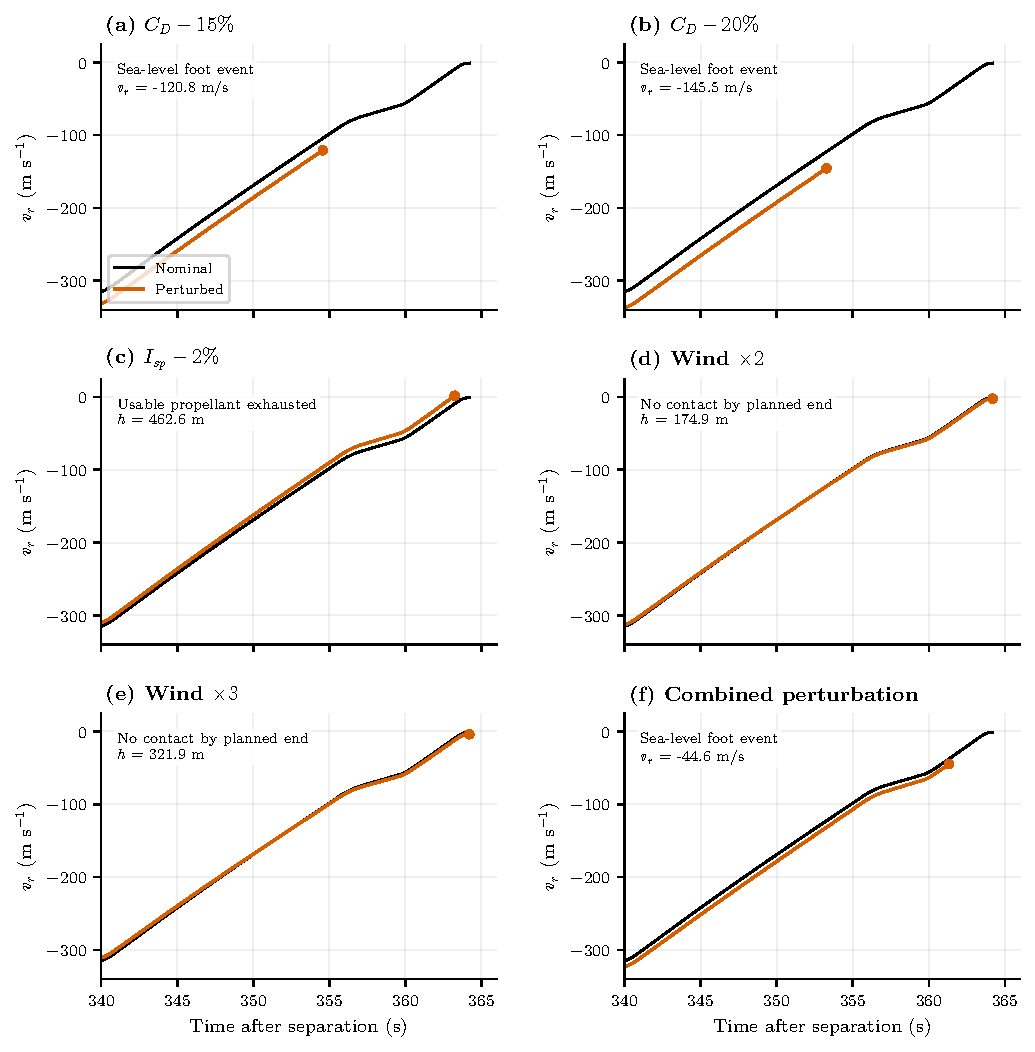
\includegraphics[width=\linewidth]{fig08_perturbations.pdf}
\caption{Late-descent radial velocity under six fixed open-loop perturbations. Every panel compares the recorded perturbation with the nominal history and stops at the case's actual terminal event. Failure can mean excessive speed, propellant exhaustion, or no contact by the planned end, rather than a single common mechanism.}
\label{fig:perturbations}
\end{figure}

All six tested cases fail the unchanged plan. Reduced drag produces rapid downward motion at the sea-level foot event and can exceed the pressure screen. Reduced specific impulse exhausts usable propellant before contact. Larger wind can leave the booster above the target height with a downrange mismatch at the planned endpoint. These are sensitivity observations for one fixed plan, not a demonstration that a redesigned feedback guidance law would fail. The cases are not random samples and supply neither a failure probability nor a propellant confidence interval.

\section{Discussion and Safety Limitations}
\label{sec:discussion}
\subsection{What the calculation establishes}
The study closes propellant accounting through a coupled trajectory and actual engine response. It distinguishes the flight-path angle from body attitude and thrust direction, uses a continuously detected foot event, and rejects an actuator violation that a finite optimization grid missed. Those steps make the numerical result more interpretable than a fuel estimate obtained from a guessed braking speed or an undocumented trigger rule.

The result nevertheless remains conditional. The verified trajectory uses $C_D=0.5$, the stated area interpolation, surrogate pressure center and inertia, and a virtual engine. Its relatively large entry-burn allocation follows both the optimized stage boundary and the imposed pressure/inflow requirements. It cannot be compared directly with an earlier short entry pulse or used to attribute a fuel difference solely to the choice of optimizer.

\subsection{Attitude authority and mass properties}
Pitch is coupled after the first ignition, but the model does not supply real mass-property histories or validated moment coefficients. A small commanded direction rate does not automatically imply adequate torque, bandwidth, or stability margin. Likewise, a first-order attitude lag or a standalone RCS rotation estimate cannot establish complete force-and-moment feasibility for the descent.

The idealized pre-ignition reference omits a real reorientation control and its mass budget. If RCS is required, its hardware mass, stored propellant, finite torque, and actual maneuver must be included consistently. Coupled six-degree-of-freedom dynamics, slosh, flexibility, and engine-out behavior remain outside the current calculation.

\subsection{First contact is not stable landing}
The nominal feet meet the stated speed, pose, and coverage screens. Their actual support forces, however, depend on leg compliance, damping, stroke, friction, deck stiffness, and ship motion, none of which has been established. At first contact the engines still produce thrust, and the cutoff tail continues to act while the legs begin to carry load.

For an ideal upright static balance, upward engine force close to weight leaves only a small normal support force and correspondingly little friction. Thus a near-upright pose and low CG speed are not sufficient anti-slide or anti-tip conditions. Engine thrust and angular rate must evolve continuously through contact rather than being set to zero. The retained reserve supports accounting for a subsequent cutoff but does not replace a support-dynamics calculation.

\subsection{Structural, thermal, and environmental limits}
Pressure and force-magnitude screens are not structural ratings. Local stress, buckling, bending, flexible response, and thermal protection depend on geometry, material properties, and distributed loads. Retropropulsion changes the engine-end flow and heating environment \cite{retro}; neither thermal integrity nor reuse readiness follows from $q<50$ kPa.

The chosen atmosphere and wind also omit date/location dependence, vertical gusts, crosswind, and sea state. The assumed high-altitude extension covers the mathematical trajectory but does not constitute a real atmospheric characterization. Robust guidance and actual recovery margins require measured or justified uncertainty models and a consistent closed-loop simulation.

\subsection{Strengths, weaknesses, and next steps}
The main strength is traceability: assumptions, candidate generation, independent replay, and unsupported recovery requirements remain separate. A second strength is the explicit force/moment and mass-flow accounting, which prevents thrust-vector prescriptions or instantaneous cutoff from silently supplying unavailable control.

The main weaknesses are the unvalidated aerodynamic and mass-property inputs, idealized pre-entry reorientation, restricted engine strategy, and local nonconvex search. The deterministic perturbation failures also show that the nominal plan cannot be reused unchanged under even the tested variations.

A defensible next step is to replace the surrogate inputs with a specified vehicle model, jointly design guidance and attitude feedback, assess fixed-ship disturbances, and simulate contact and shutdown through a defined support interval. Only candidates satisfying the same complete requirements should then be compared for propellant efficiency.

\section{Conclusion}
\label{sec:conclusion}
For an upward $45^\circ$ separation at 70 km, a seven-engine virtual booster with the stated drag, wind, and actuator assumptions admits a verified nominal candidate carrying \Load\ t of total propellant. Entry and shutdown tail consume \EntryFuel\ t, and the final burn consumes \LandingFuel\ t. First foot contact occurs after \FlightTime\ s at a surface range of \Range\ km, with approximately 1 m/s downward speed. Maximum dynamic pressure is \PeakQ\ kPa.

Independent coordinate, atmosphere, response, and integration checks support this numerical benchmark. Continuous replay also identifies and resolves an inter-node thrust-slew violation. However, all six tested fixed open-loop perturbations fail, and true propulsion, aerodynamics, mass properties, three-dimensional motion, structure, heating, and support dynamics remain unresolved. The defensible conclusion is a conditional nominal propellant estimate and a defined completion path, not a global minimum or a verified robust shipboard recovery load.

\clearpage
\appendix
\section{Additional Model and Acceptance Details}
\subsection{Atmospheric layers and boundary treatment}
The lower-atmosphere geopotential boundaries are 0, 11, 20, 32, 47, 51, 71, and 84.852 km. Temperature gradients are $-6.5$, 0, 1, 2.8, 0, $-2.8$, and $-2$ K/km. Sea-level values are 288.15 K and 101,325 Pa. The extension in \cref{eq:extension} starts at the geometric height corresponding to the final geopotential boundary. Its density is continuous there; its assigned scale height is a separate H choice.

\subsection{Engine and support geometry}
The engine allocation in \cref{eq:allocation} uses a 2.5 m ring radius and 32.5 m axial lever. All thrust directions are parallel in each allocation state, so the total magnitude $T$ also determines mass flow. If a future model gives engines independent directions, translation must use the vector sum while mass flow remains tied to the sum of individual thrust magnitudes.

The 65 m envelope, 2 m basal gap, and equivalent-cylinder inertia should not be interpreted as a fully specified vehicle layout. They jointly define the present surrogate. The actual center of mass can differ from a geometric midpoint and can migrate as propellant is consumed; the corresponding internal-flow and inertia terms would need to be rederived for a real mass distribution.

\subsection{Nominal event and numerical tolerances}
Replay terminates at first deployed-foot sea-level contact or unusable-propellant exhaustion. For the nominal event, the ship's center is selected at the nominal CG surface projection. The finite deck and body-envelope screens are then evaluated. Far from the ship, the global surface is spherical, not an infinite extension of the local tangent plane.

Nominal root bracketing permits no more than 0.05 s beyond the planned end solely to locate a small numerical event discrepancy. Perturbation cases stop at the planned end without such control extension. The quoted step-halving comparisons concern the fixed recorded controls, not the completeness of a continuous-time safety proof.

\section{Computational Traceability}
\label{app:reproduction}
The typeset results use a frozen record of the verified computation. This manuscript-generation step does not rerun trajectory optimization or modify the dynamics. The accompanying reproduction bundle supplies the numerical summary, actual control arrays, nominal and perturbed replay arrays, generated table rows, and the scripts that rebuild the figures and numerical macros. A separate lightweight LaTeX package supplies the ready-to-use vector figures and generated rows needed for compilation.

The simulation record uses Python 3.12.14, CasADi 3.7.2 with IPOPT, NumPy 2.3.5, and SciPy 1.17.0. Important evidence files include \texttt{metrics.json}, \texttt{verification.json}, \texttt{physics\_checks.json}, \texttt{optimized\_controls.npz}, and \texttt{fixed\_control\_perturbations.csv}. The record distinguishes returned local candidates, iteration-limited searches, rejected slew histories, and resource-terminated runs.

The paper is compiled with XeLaTeX and BibTeX. All eight main figures are vector PDFs, with consistent panel labels, units, and annotations. They are regenerated from the archived data; no numerical curve or substantive text from the reference example papers is reused.

\clearpage
\phantomsection
\addcontentsline{toc}{section}{References}
\bibliographystyle{unsrt}
{\small\bibliography{references}}

\clearpage
\section*{Report on the Use of AI}
\addcontentsline{toc}{section}{Report on the Use of AI}
\noindent\textbf{Draft disclosure status: incomplete; not a submission-ready record.}

ChatGPT, through a Codex workspace assistant, assisted with the associated modeling, programming, numerical checks, editorial revision, figure generation, and LaTeX manuscript preparation. The exact underlying model release has not been verified and is not invented here. The present verified manuscript request was:
\begin{quote}
{\zhfont\small\XeTeXlinebreaklocale "zh"\XeTeXlinebreakskip=0pt plus 1pt
参照这篇论文的结构和框架和文章格式，字体大小，图片形式和标注，去用LateX写论文}
\end{quote}
The competition rules request the system identity, exact queries, and complete outputs when generative AI is used \cite{rules}. The single quoted request and the source code are not a verbatim record of all previous interactions. Complete prompts and full outputs from modeling, revision, and this manuscript step must be assembled from the actual session records before submission; missing records must not be reconstructed as though they were exact. The team must independently review all AI-produced physics, calculations, wording, and references. The team number remains a placeholder.
\end{document}
